\documentclass[tikz]{standalone}
\usepackage{amsmath}
\usepackage{xcolor}
\usetikzlibrary{arrows.meta,shapes.geometric,positioning,calc}

% 颜色
\definecolor{blk}{HTML}{000000}

% 统一样式
\tikzset{
  arr/.style = {
    -{Stealth[length=3.4pt,width=6pt]},
    line width=0.8pt, draw=blk
  },
  amp/.style = {
    isosceles triangle, shape border rotate=90,
    minimum width=18mm,   % 底边(在左)
    minimum height=14mm,  % 高度(尖端朝右)
    inner sep=0pt,
    draw=none, fill=blk,
    text=white, font=\rmfamily\small, align=center
  },
  bs/.style = {
    rectangle,
    minimum width=7mm,
    minimum height=42mm,
    inner sep=0pt,
    draw=none, fill=blk,
    text=white, font=\rmfamily\small, align=center
  },
  lab/.style = {font=\normalsize, inner sep=1pt}
}

\begin{document}
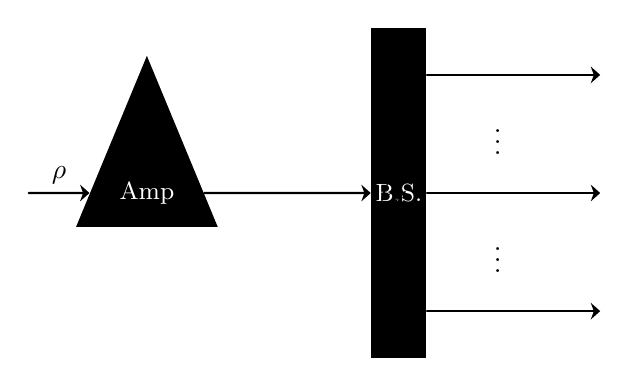
\begin{tikzpicture}[x=1cm,y=1cm,line cap=round,line join=round]

  % 位置基准
  \coordinate (inL) at (-3.0,0);         % 输入线起点
  \node[amp] (amp) at (-1.5,0) {Amp};    % 放大器
  \node[bs]  (bs)  at ( 1.7,0) {B.S.};   % 黑色矩形

  % 输入箭头与标签 ρ
  \draw[arr] (inL) -- (amp.west)
    node[midway,above=2pt,lab] {$\rho$};

  % 放大器 -> B.S.
  \draw[arr] (amp.east) -- (bs.west);

  % 输出(等间距三路)
  \foreach \yy/\labtext in {1.5/{\rho_1}, 0/{\rho_\mu}, -1.5/{\rho_N}}{
    % 箭头
    \draw[arr] (bs.east)++(0,\yy) -- ++(2.2,0);
    % 标签放在输出起点的左侧略偏右(避免压到矩形)
    \node[lab,anchor=east] at ($(bs.east)+(-0.18,\yy)$) {$\labtext$};
  }

  % 竖向省略(可用单个或多个 \vdots)
  \node[lab] at ($(bs.east)+(0.9,0.75)$) {$\vdots$};
  \node[lab] at ($(bs.east)+(0.9,-0.75)$) {$\vdots$};

\end{tikzpicture}
\end{document}